\fontsize{13px}{13px}\selectfont\justifying

\subsection{Kết quả}
\subsubsection{Môi trường \Gls{staging}}
\FloatBarrier
\begin{figure}[!htbp]\fontsize{13px}{13px}\selectfont
\centering
		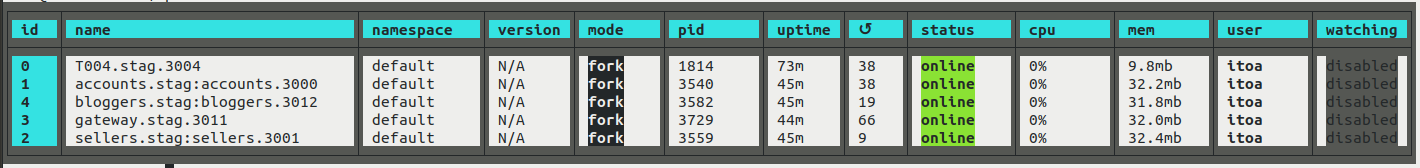
\includegraphics[width=\textwidth]{./results/vps-staging}
		\caption{Thông tin các tiến trình máy chủ \gls{staging}}
\justifying
Xem kết quả ứng dụng web tại fashion.ocopee.com
\end{figure}
\subsubsection{Môi trường \Gls{production}}
\FloatBarrier
\begin{figure}[!htbp]\fontsize{13px}{13px}\selectfont
\centering
		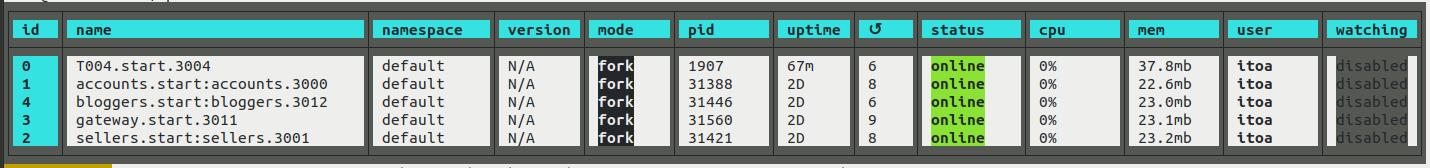
\includegraphics[width=\textwidth]{./results/vps-production}
		\caption{Thông tin các tiến trình máy chủ \gls{production}}
\justifying
Xem kết quả ứng dụng web tại ocopee.com
\end{figure}
\FloatBarrier
\begin{figure}[!htbp]\fontsize{13px}{13px}\selectfont
\centering
		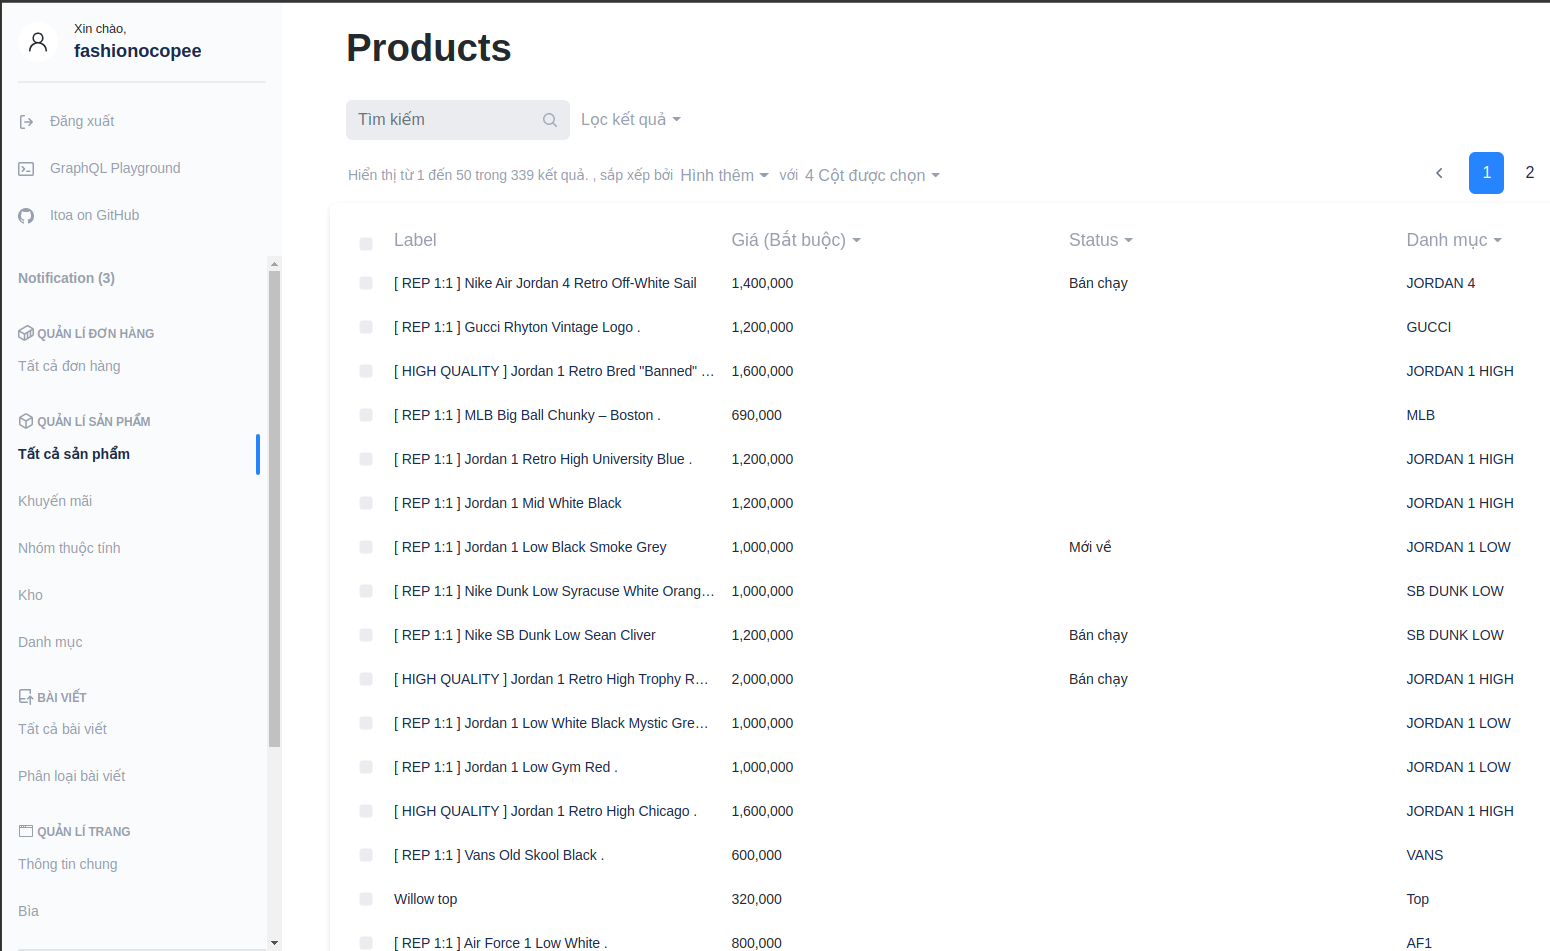
\includegraphics[width=\textwidth]{./results/product}
		\caption{Trang quản lí sản phẩm}
\justifying
\end{figure}
\clearpage
\subsubsection{Trang quản lí đơn hàng}
\FloatBarrier
\begin{figure}[!htbp]\fontsize{13px}{13px}\selectfont
\centering
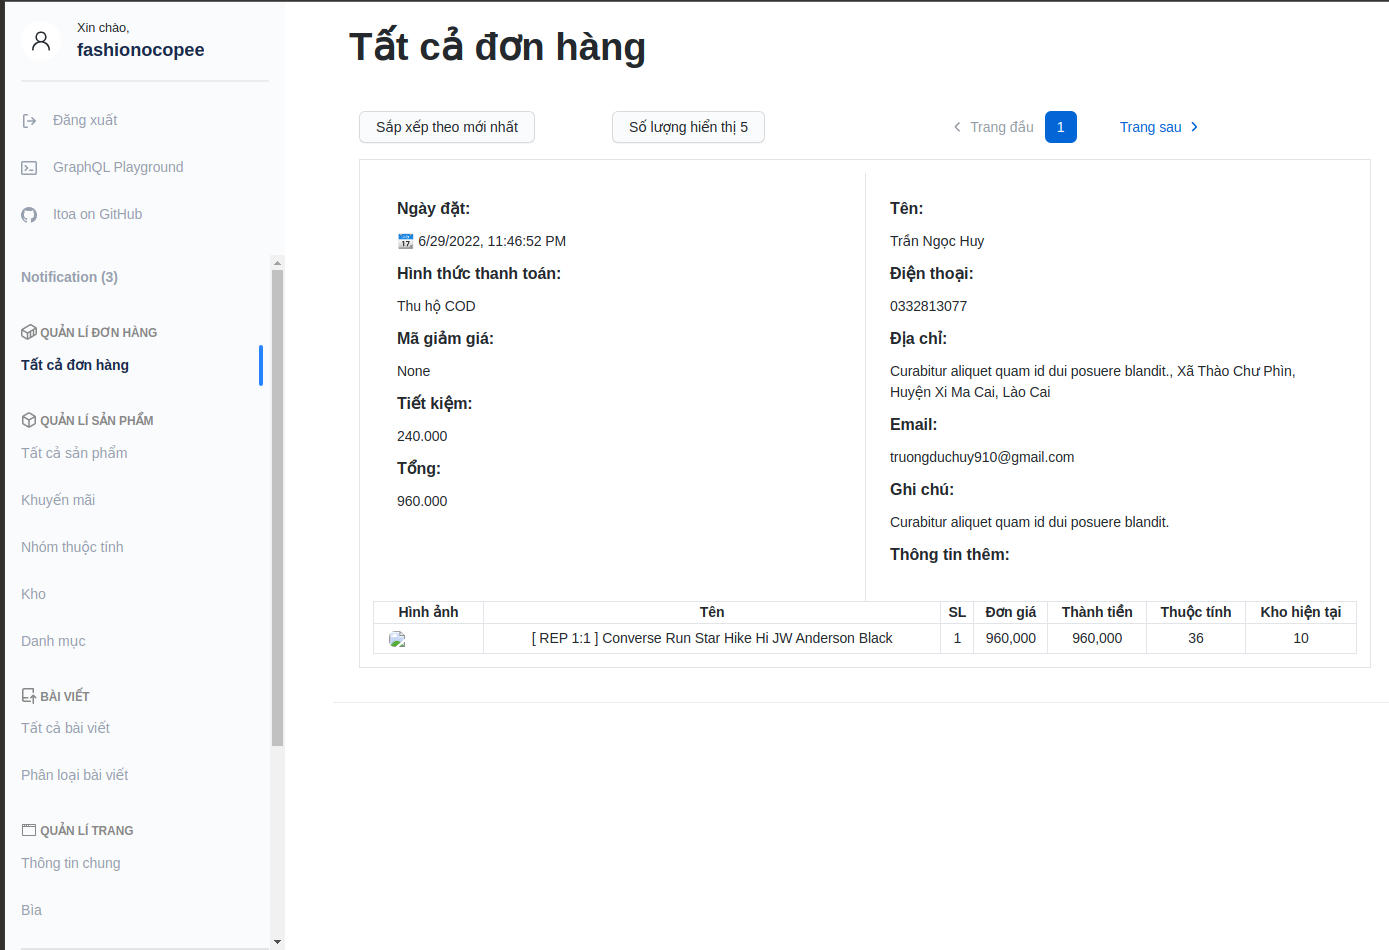
\includegraphics[width=\textwidth]{./results/order}
\caption{Trang quản lí đơn hàng}
\justifying
Trang quản lí thông tin đơn hàng dành cho nhà bán hàng cho phép nhà bán hàng xem thông tin người mua hàng để lại bao gồm: Địa chỉ nhận hàng, thông tin liên hệ, hình thức thanh toán, chi tiết đơn hàng và mã giảm giá đã sử dụng.
\end{figure}
\clearpage
\subsubsection{Trang kết bạn và chia sẻ sản phẩm}
\FloatBarrier
\begin{figure}[!htbp]\fontsize{13px}{13px}\selectfont
\centering
		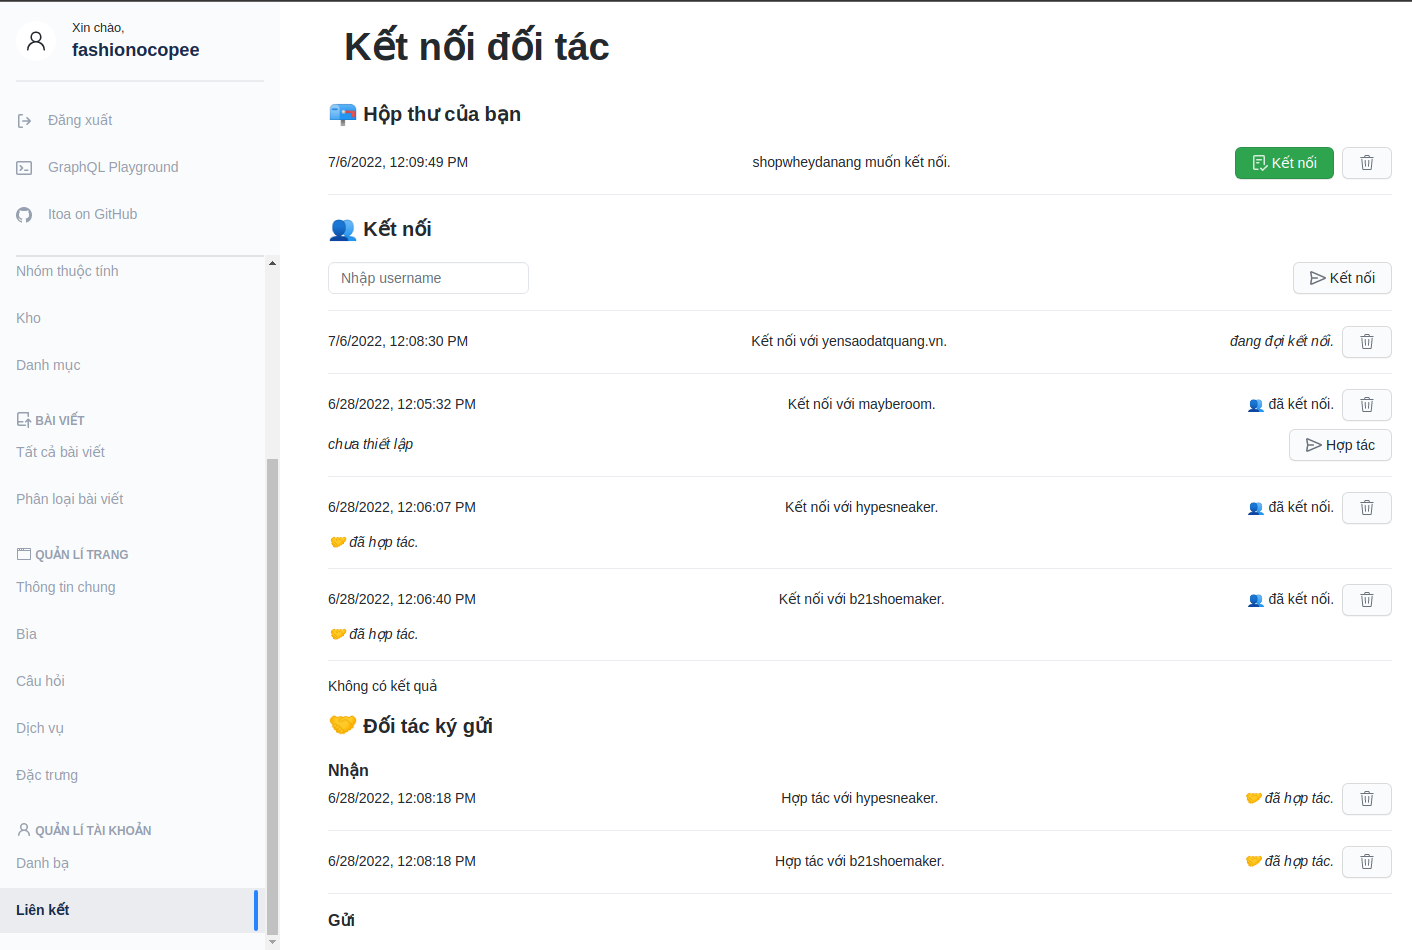
\includegraphics[width=\textwidth]{./results/contract}
		\caption{Trang kết bạn và chia sẻ sản phẩm}
\justifying
Tính năng kết bạn và chia sẻ sản phẩm được trình bày dưới dạng kết nối và ký gửi, theo cách gọi thông thường của nhà sản xuất và cửa hàng. Trước khi gửi hoặc nhận dữ liệu từ đối tác. Hai bên cần gửi lời mời kết bạn cho nhau và không quan trong người nào gửi cho người nào.

Riêng với tính năng hợp tác, người tạo yêu cầu chia sẻ sản phẩm. Tức là người bấm vào nút hợp tác trên một dòng trong danh sách đã kết nối. Người yêu cầu là người được quyền xem và trình bày thông tin sản phẩm của đối tác lên trang của mình.

Đồng nghĩa với việc, nếu nhà sản xuất chấp nhận lời mời, sản phẩm của họ sẽ được hiển thị và đăng bán trên trang của người tạo ra lời mời hợp tác.
\end{figure}
\clearpage
\subsubsection{Trang thông báo}
\FloatBarrier
\begin{figure}[!htbp]\fontsize{13px}{13px}\selectfont
\centering
		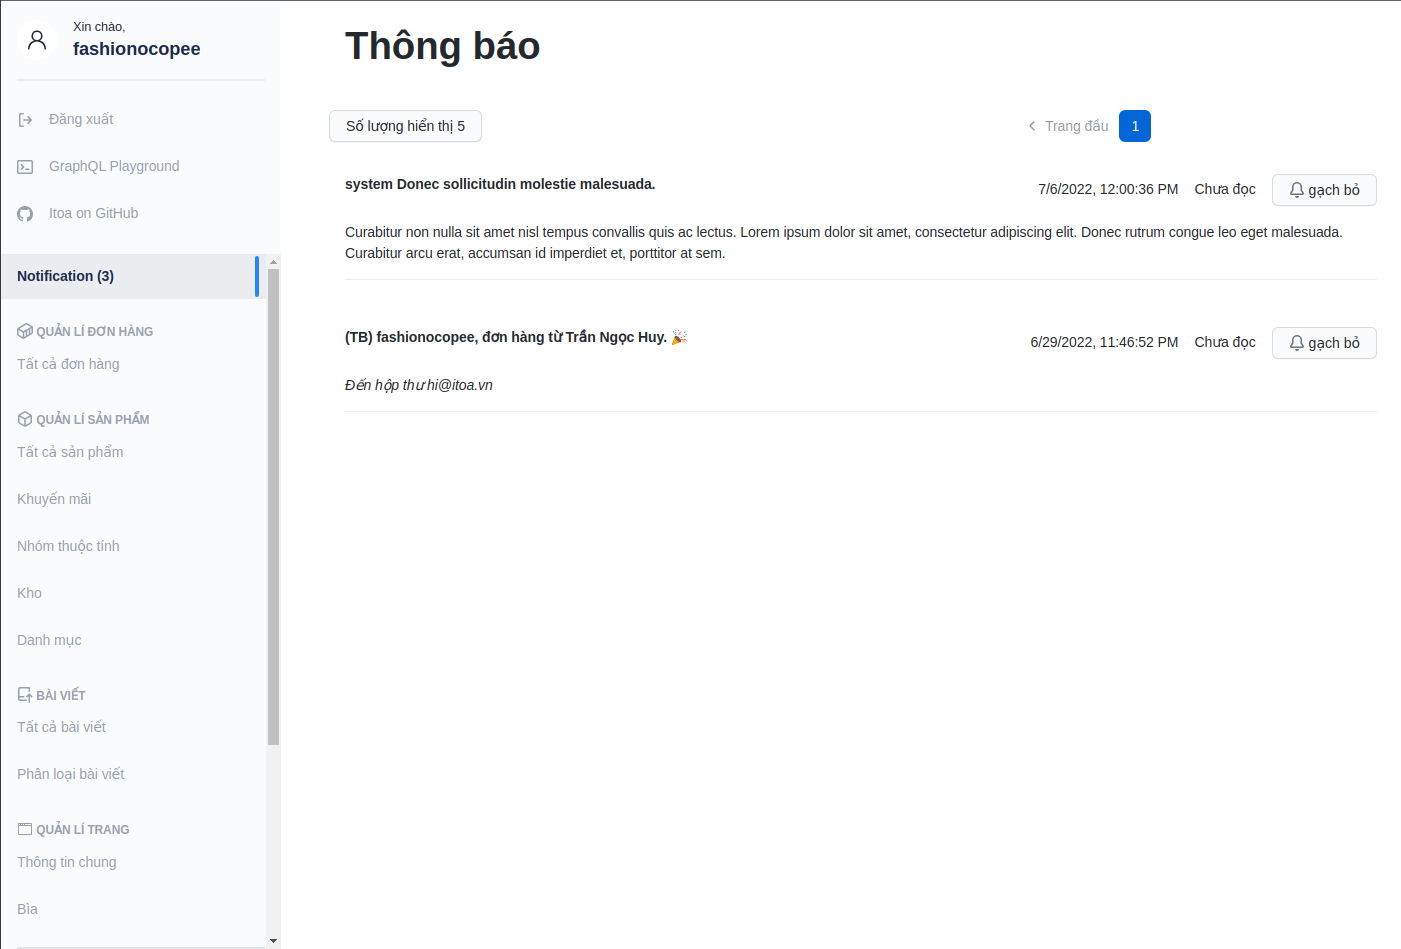
\includegraphics[width=\textwidth]{./results/notifications}
		\caption{Trang thông báo}
\justifying
Trang thông báo giúp cho nhà bán hàng hoặc nhà sản xuất kiểm tra hộp thư thông báo của mình. Đánh dấu các thông báo đã xem. Trang thông báo mặc định hiển thị ưu tiên các thông báo mới nhất chưa được xem.

Các thông báo đến địa chỉ thư điện tử của nhà bán hàng sẽ không được hiển thị nội dung mà thay vào đó. Thông báo chỉ hiển thị thông tin tiêu đề và ghi chú kiểm tra hộp thư.
\end{figure}
\clearpage
\subsubsection{Trang quản lí danh mục}
\FloatBarrier
\begin{figure}[!htbp]\fontsize{13px}{13px}\selectfont
\centering
		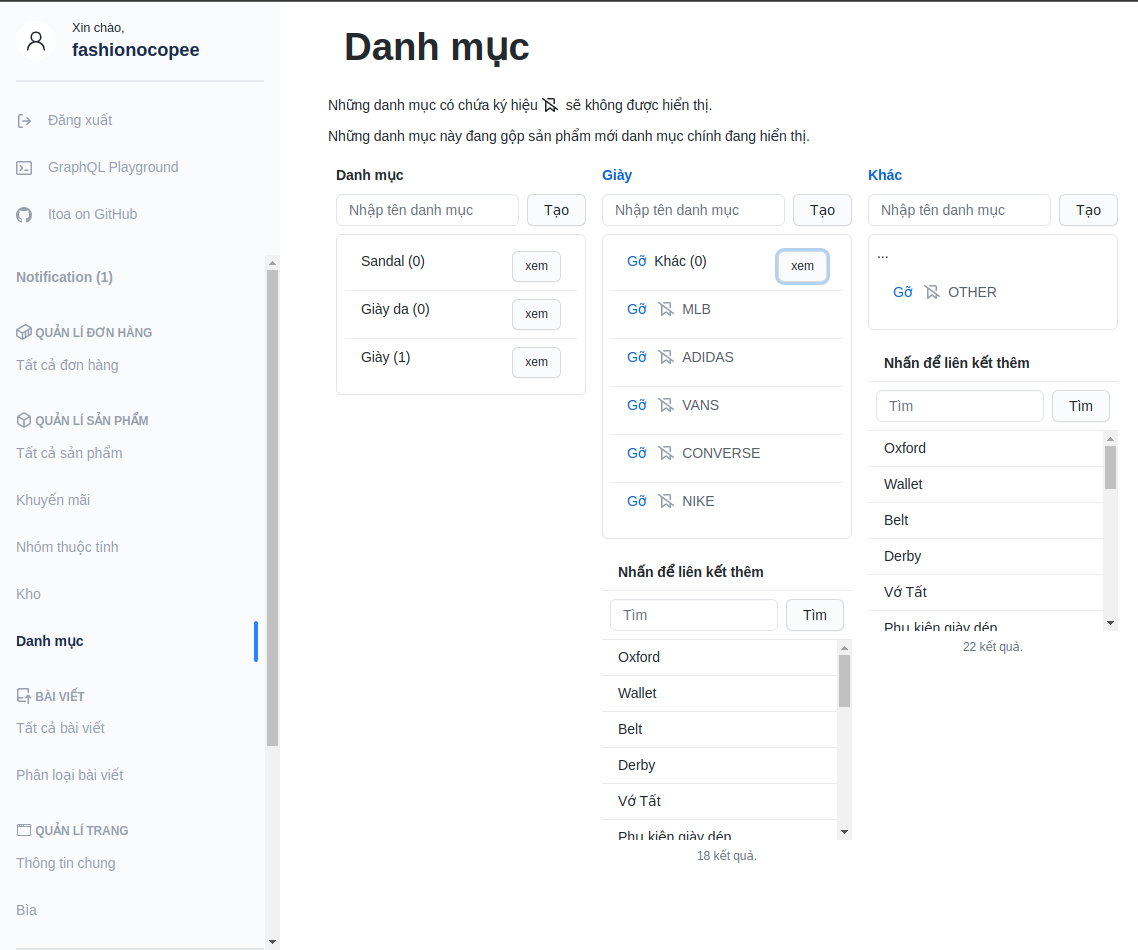
\includegraphics[width=\textwidth]{./results/categories}
		\caption{Trang quản lí danh mục}
\justifying
Quản lý danh mục giúp phân loại sản phẩm cho nhà sản xuất. Khi chia sẻ cho các nhà bán hàng. Danh mục sản phẩm có chức năng đánh dấu danh mục tương đương.

Nghĩa là đối với một nhà sản xuất hoặc nhà bán hàng. Họ luôn có cho mình cây danh mục do họ sở hữu. Và cũng là cây danh mục hiển thị chính trên trang.

Nhưng khi được chia sẻ sản phẩm, các sản phẩm được chia sẻ được liên kết với danh mục của nhà sản xuất. Và các danh mục ngoài nằm ngoài quyền quản lí của nhà bán hàng. Do vậy, tính năng danh mục tương đương đánh dấu các danh mục nào của nhà sản xuất là tương đương với danh mục của nhà bán hàng hiện tại. Sau khi đánh dấu tương được thì sản phẩm của nhà sản xuất, mặc dù nằm ngoài quyền quản lí của nhà bán hàng nhưng cũng có thể sắp xếp tìm kiếm bởi danh mục riêng của nhà bán hàng.
\end{figure}
\clearpage
\subsubsection{Trang quản lí tồn kho}
\FloatBarrier
\begin{figure}[!htbp]\fontsize{13px}{13px}\selectfont
	\centering
		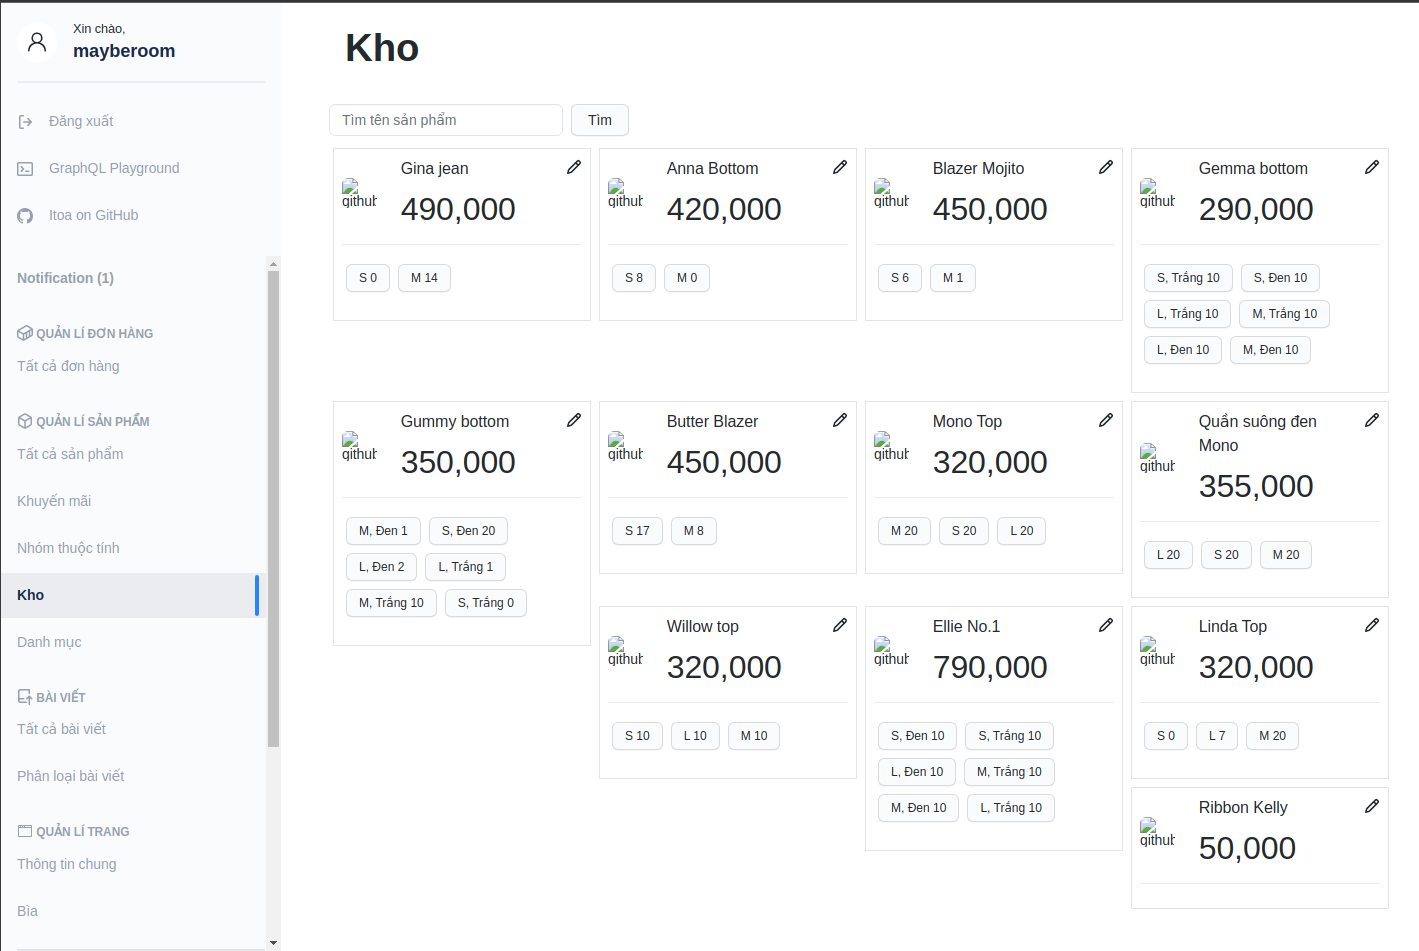
\includegraphics[width=\textwidth]{./results/stock}
		\caption{Trang quản lí tồn kho}
	\justifying
Quản lí có chức năng hiển thị tồn kho khi khách hàng chọn thuộc tính của sản phẩm. Ngăn chặn người dùng thêm nhiều hơn số tồn kho vào giỏ hàng hoặc mua sản phẩm hết hàng. Quản lí kho không bao gồm các chức năng tự động giảm số lượng trong kho khi đơn hàng sử lý thành công.
\end{figure}
\clearpage
\subsubsection{Trang quản lí thuộc tính}
\FloatBarrier
\begin{figure}[!htbp]\fontsize{13px}{13px}\selectfont
\centering
		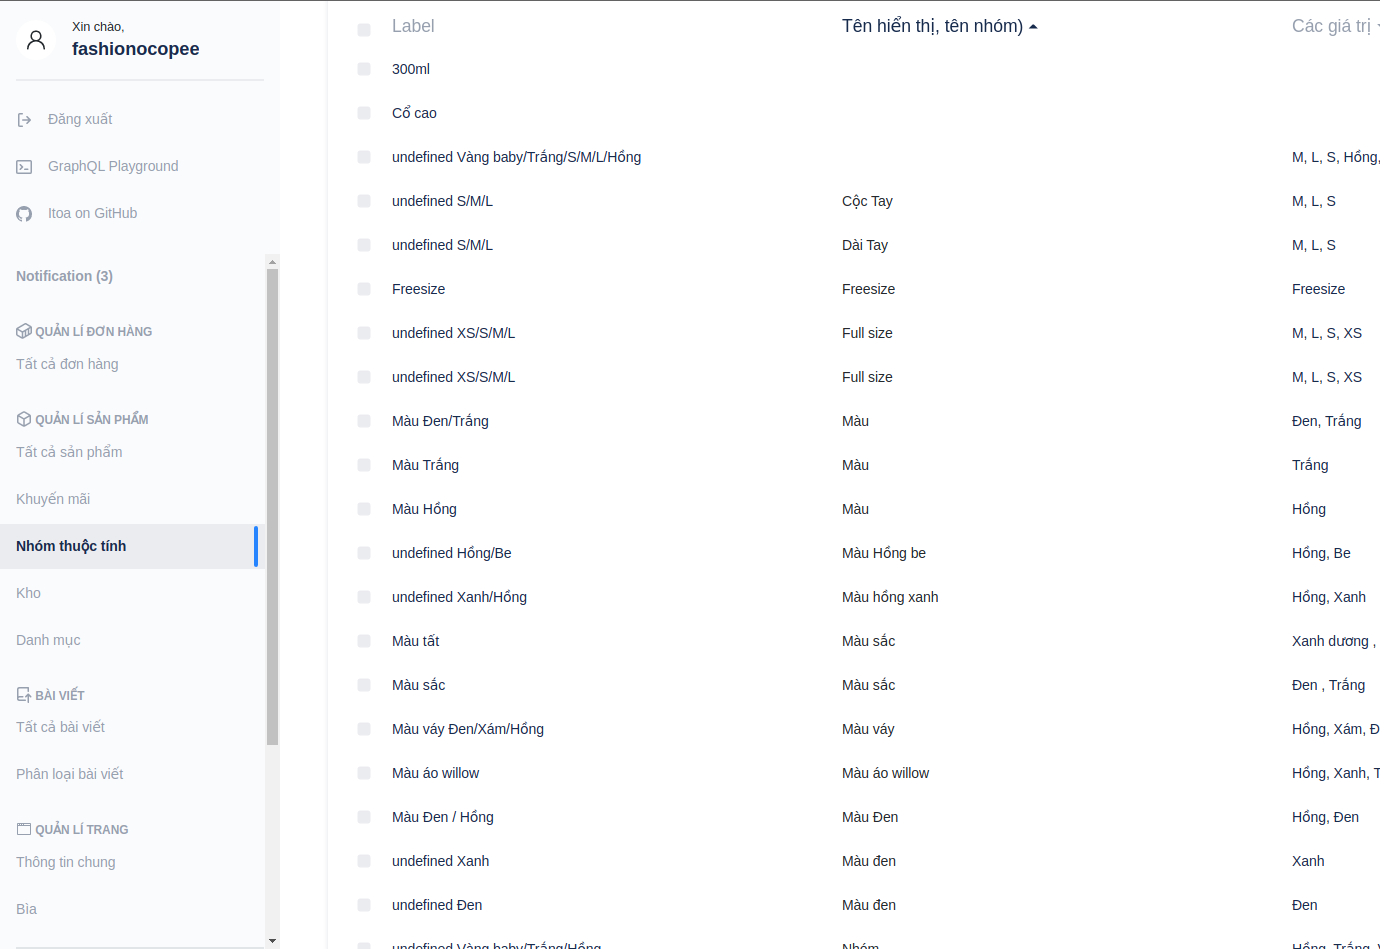
\includegraphics[width=\textwidth]{./results/attributes}
		\caption{Trang quản lí thuộc tính}
\justifying
Thuộc tính của một sản phẩm được định nghĩa là các phiên bản khác nhau của sản phẩm đó. Cùng một quy trình sản xuất hoặc cùng giá bán và chi phí sản xuất có thể cho là cùng một sản phẩm. Các thuộc tính của sản phẩm cũng được nhóm, quản lý kho và hình ảnh của thuộc tính đó. Ví dụ: kích thước, màu sắc. Cùng một sản phẩm giày nhưng khác màu sắc thì hình ảnh hiển thị cũng cần được lưu trữ và hiển thị trên trang.
\end{figure}
\clearpage
\subsubsection{Trang quản lí thông tin cửa hàng}
\FloatBarrier
\begin{figure}[!htbp]\fontsize{13px}{13px}\selectfont
\centering
		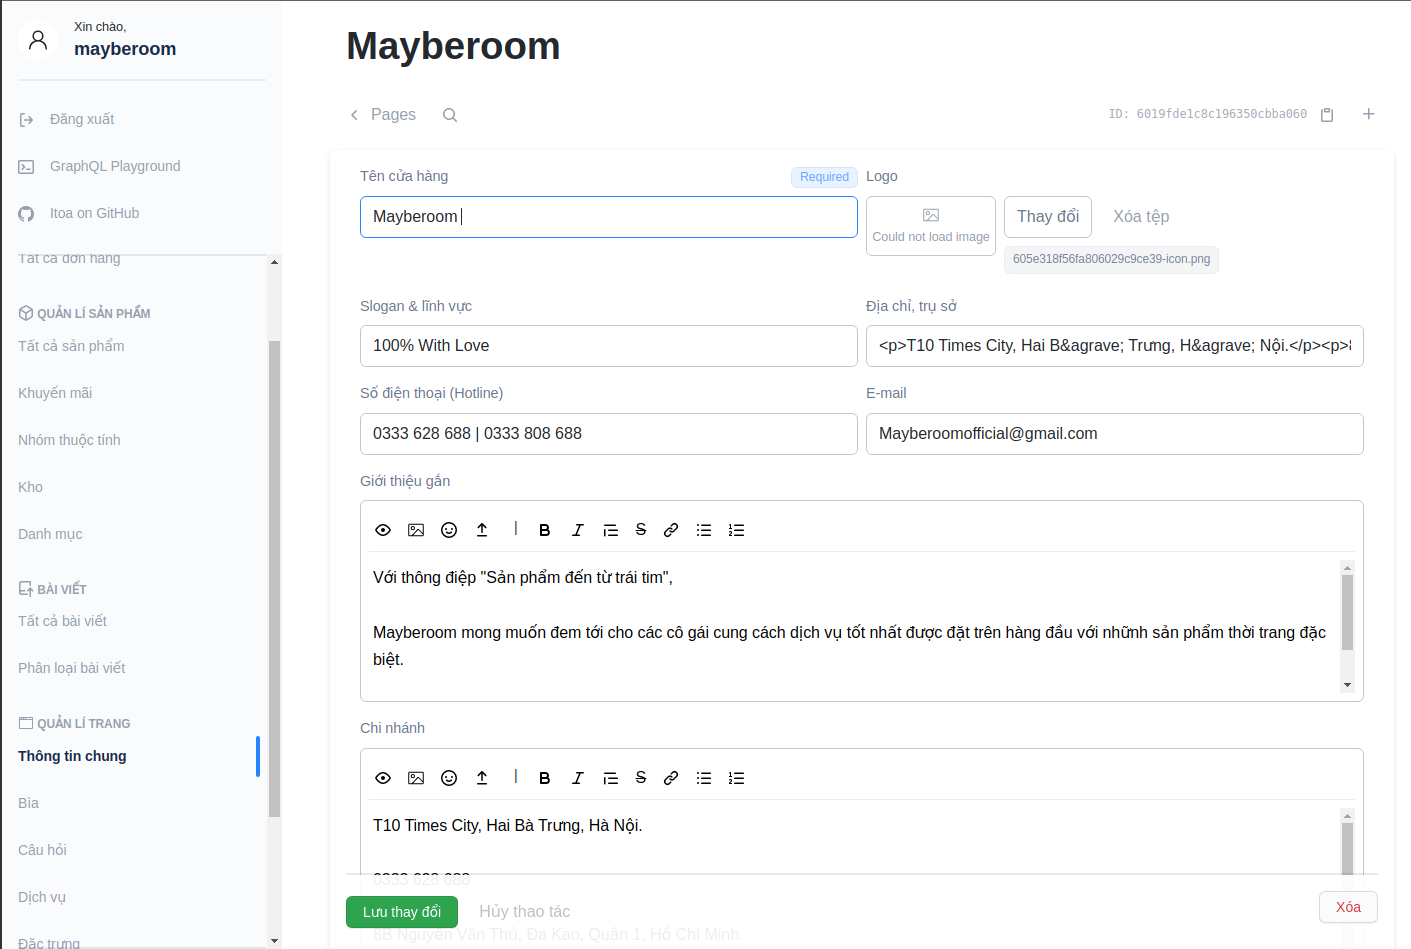
\includegraphics[width=\textwidth]{./results/store}
		\caption{Trang quản lí thông tin cửa hàng}
\justifying
Trang quản lý cửa hàng bao gồm các thông tin liên hệ cơ bản của nhà bán hàng. Các chính sách như thanh toán và vận chuyển.

Quản lí cửa hàng cũng bao gồm các thông tin thiết kế, tùy biến cá nhân hóa cho từng nhà bán hàng. Ví dụ như: Màu chủ đạo, lời chào,...
\end{figure}
\clearpage
\subsubsection{Trang quản lí mã giảm giá}
\FloatBarrier
\begin{figure}[!htbp]\fontsize{13px}{13px}\selectfont
\centering
		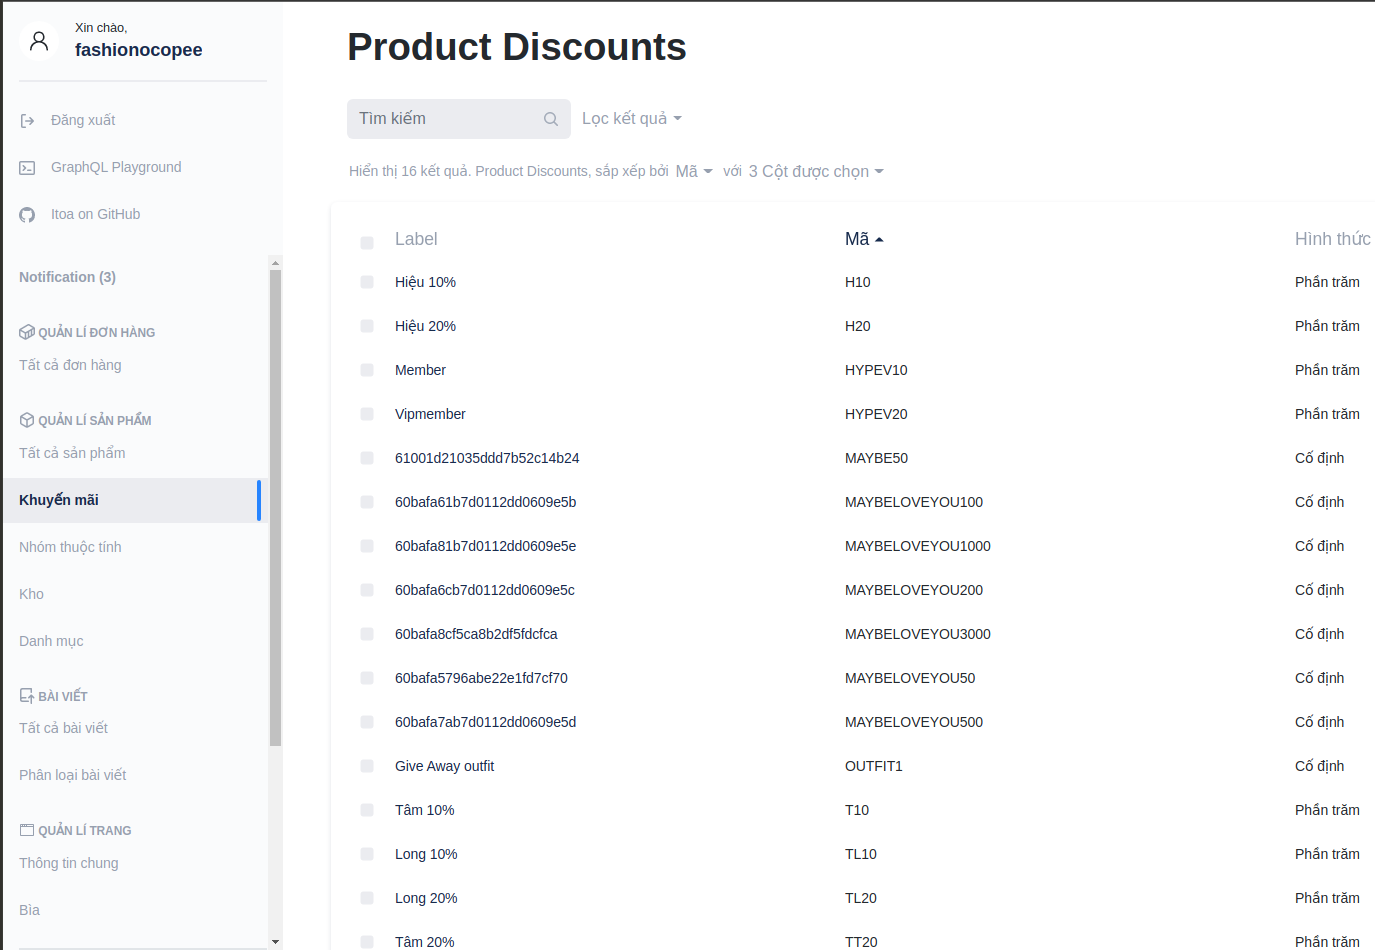
\includegraphics[width=\textwidth]{./results/discount}
		\caption{Trang quản lí mã giảm giá}
\justifying
	Trang quản lí mã khuyến mãi giúp người quản trị xem, sửa, xóa các mã khuyến mãi dựa theo phần trăm giảm. Hoặc theo giá cố định. Mã khuyến mãi cũng có thể đặt điều kiện tối thiểu để áp dụng mã giảm giá.
	
	Mã giảm giá của nhà sản xuất có thể được chia sẻ cho nhà bán hàng nhưng không thể sử dụng bởi một nhà sản xuất khác cũng cùng cung cấp sản phẩm cho nhà bán hàng.

	Mặc định mã giảm giá không thể truy cập bởi khách hàng, thông qua phiếu đặt hàng, mã giảm giá được nhập vào và kiểm tra trên hệ thống máy chủ.
\end{figure}
\clearpage
\subsubsection{Trang chủ sàn thương mại điện tử}
\FloatBarrier
\begin{figure}[!htbp]\fontsize{13px}{13px}\selectfont
\centering
		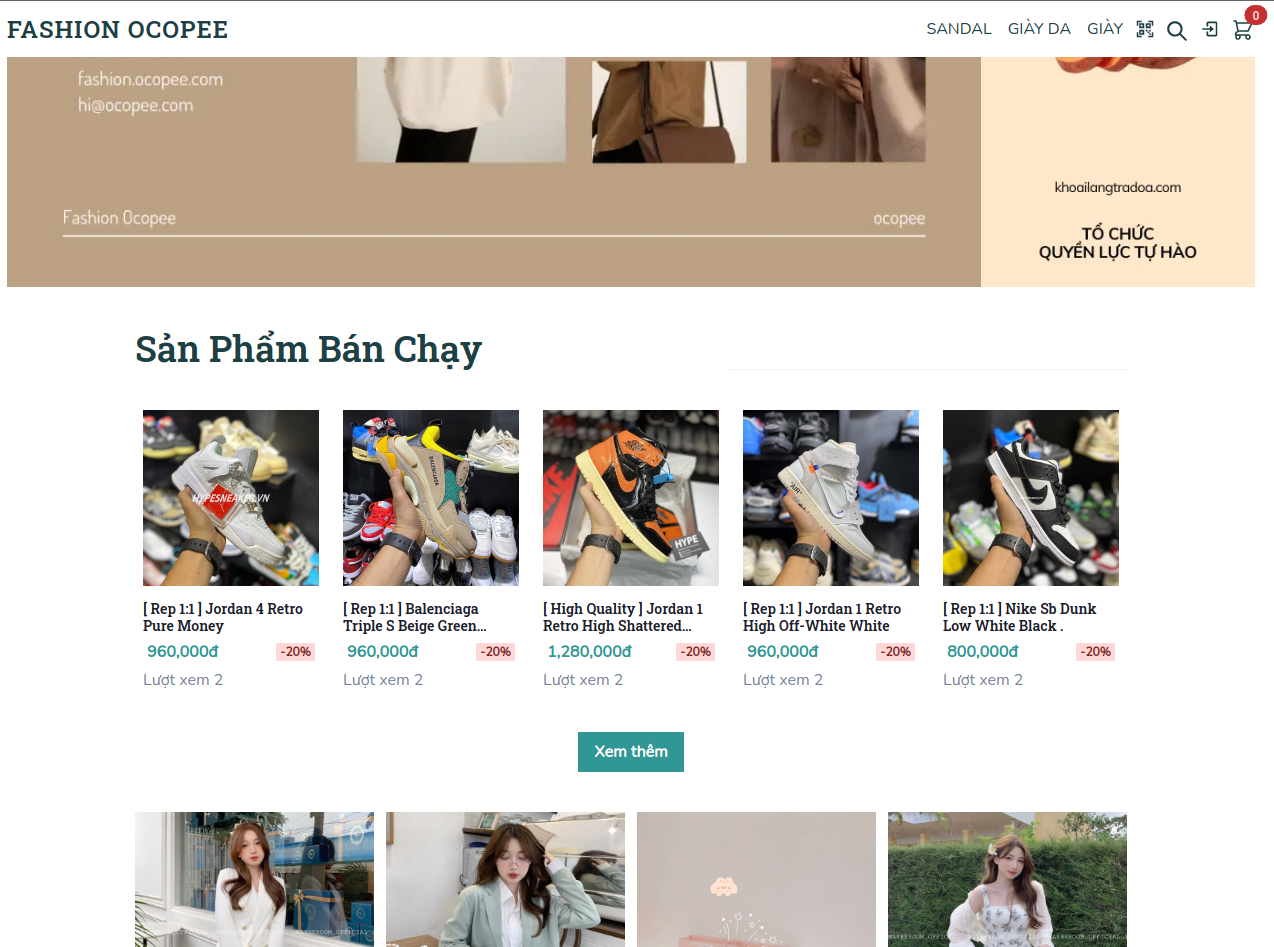
\includegraphics[width=\textwidth]{./results/homepage}
		\caption{Trang chủ sàn thương mại điện tử}
\justifying
Trang chủ sàn thương mại điện tử cho nhà bán hàng hiển thị các thông tin sản phẩm được chia sẻ cho sàn. Các hình ảnh quảng cáo. Điều hướng đến trang danh mục và chi tiết sản phẩm.
\end{figure}
\clearpage
\FloatBarrier
\begin{figure}[!htbp]\fontsize{13px}{13px}\selectfont
\centering
		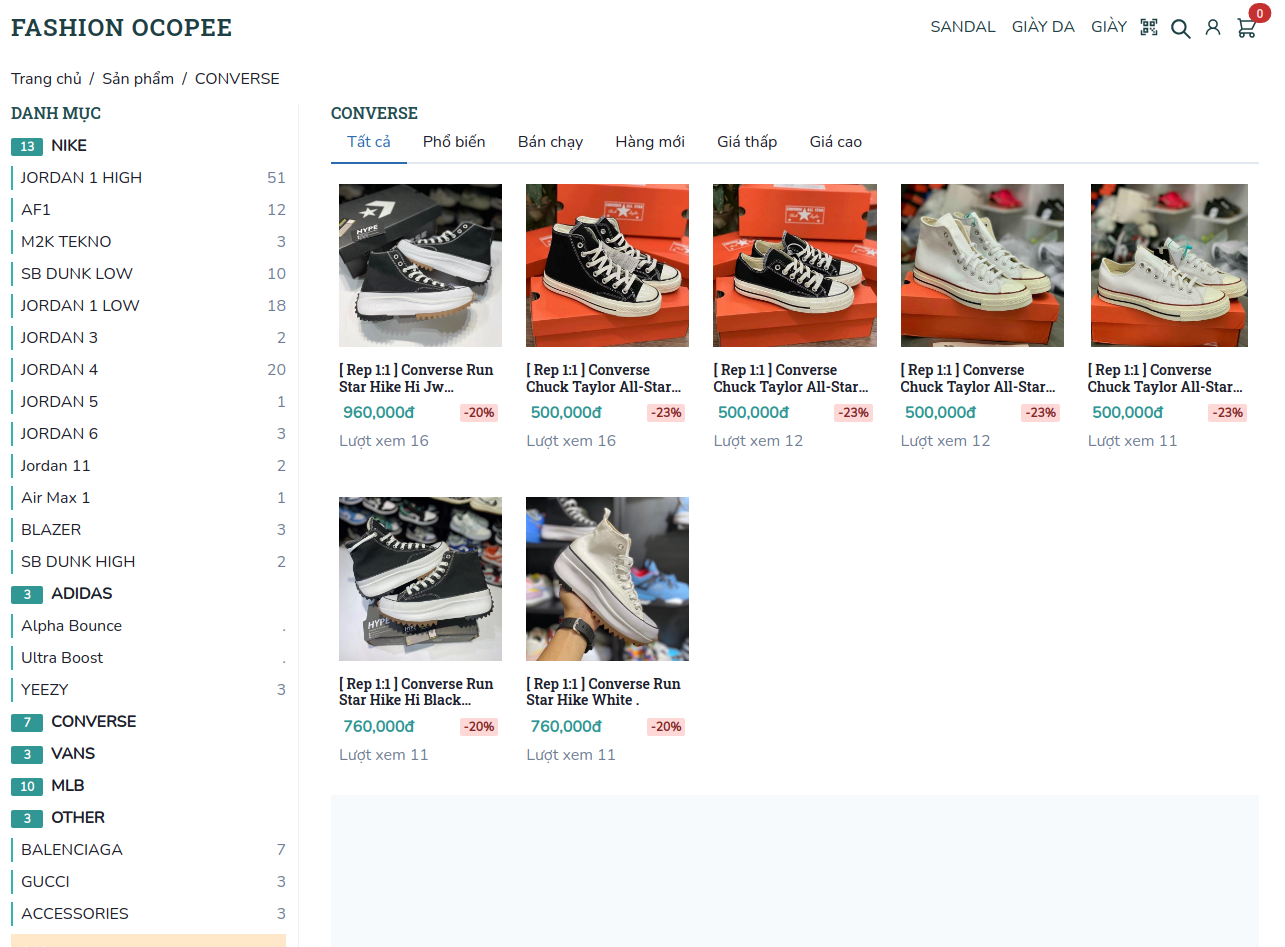
\includegraphics[width=\textwidth]{./results/categories-page}
		\caption{Trang duyệt xem sản phẩm}
\justifying
Trang duyệt xem hay còn gọi là trang trình bày sản phẩm, danh mục sản phẩm chung được quản lí bởi nhà bán hàng. Người dùng có thể xem sản phẩm theo danh mục, với các trạng thái như: bán chạy, phổ biến, hàng mới, giá thấp, giá cao... Nút xem thêm sản phẩm được thiết kế theo kiểu nối thêm sản phẩm thay vì lật trang.

\end{figure}
\clearpage
\FloatBarrier
\begin{figure}[!htbp]\fontsize{13px}{13px}\selectfont
\centering
		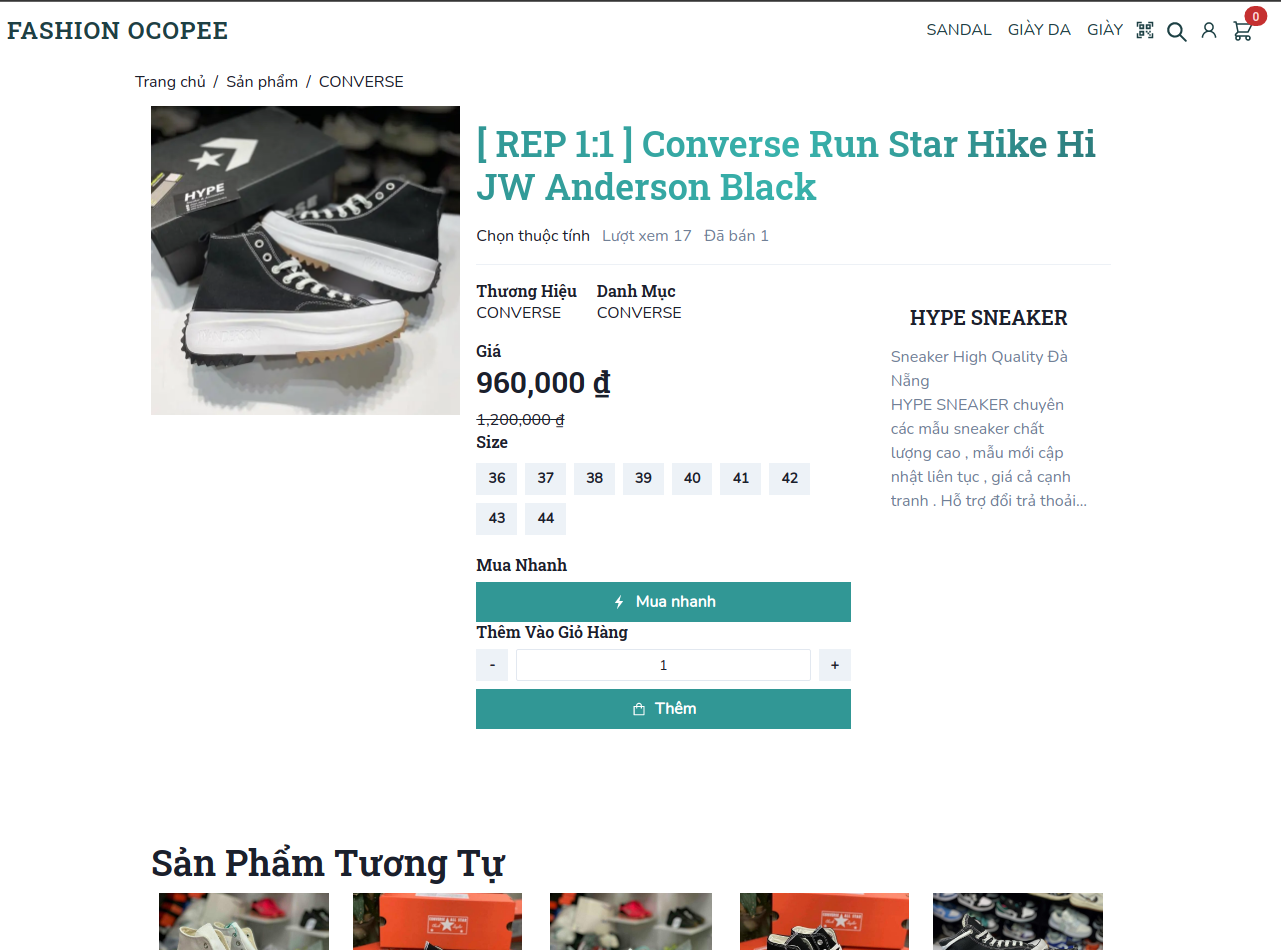
\includegraphics[width=\textwidth]{./results/product-page}
		\caption{Trang chi tiết sản phẩm}
\justifying
Trang chi tiết sản phẩm cho phép người mua hàng lựa chọn các thuộc tính của sản phẩm. Xem tồn kho của thuộc tính đó. Chức năng mua nhanh cho một sản phẩm duy nhất vào giỏ hàng và điều hướng đến trang thông tin đặt hàng. Chức năng thêm sẽ thêm số lượng sản phẩm tương ứng vào giỏ hàng. Bên cạnh thông tin chi tiết có hiển thị thông tin nhà cung cấp hoặc nhà sản xuất. Người dùng có thể đi đến không gian riêng của từng nhà sản xuất, trong trang chung hiện tại.
\end{figure}
\clearpage
\FloatBarrier
\begin{figure}[!htbp]\fontsize{13px}{13px}\selectfont
\centering
		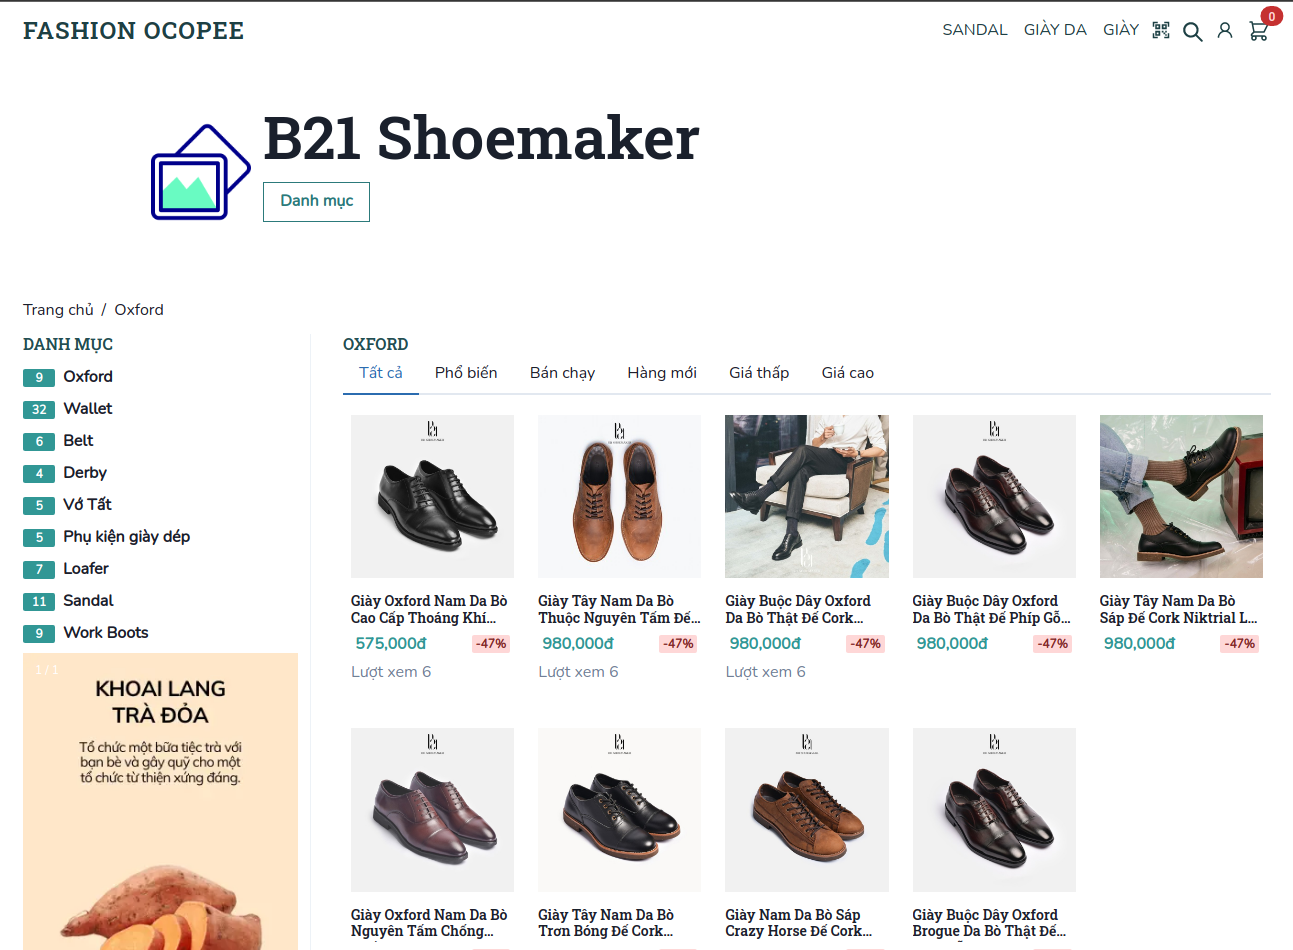
\includegraphics[width=\textwidth]{./results/store-page}
		\caption{Trang riêng của từng nhà sản xuất trên sàn}
\justifying
	Từng nhà sản xuất khi tham gia chia sẻ sản phẩm lên trang chung của nhà bán hàng cũng được xây dựng một không gian gian hàng riêng.
	Khác với trình bày sản phẩm chung, trang trình bày sản phẩm riêng cho từng nhà cung cấp, nhà sản xuất sử dụng danh mục sản phẩm được tạo ra bởi chính nhà sản xuất đó.
\end{figure}